\part{Introduction}
\label{partIntroduction}

Injuries that occur after blast or non-penetrating ballistic projectile impacts to a soldier wearing Personal Protective Equipment (PPE) are referred to as Behind Armor Blunt Trauma (BABT).  The kinetic energy from such an impact is absorbed by the soldier's PPE, and by the bony and soft tissues of the soldier beneath.  Standards have been written by which PPE's have been designed to since 1972.  Verification is through experiments where, typically, a suit of body armor is placed over a `body' subjected to a ballistic impact from a projectile fired by a weapon, all in accordance with a standard.  Current practice is to use clay (usually Roma Plastilina No.~1 clay) as a surrogate for the human body in these tests.  A principle objective of an internal Army Research Laboratory--Weapons and Materials Research Directorate (ARL-WMRD) project, \textit{Modeling Large Deformations and Stress Wave Mechanics in Soft Biological Tissue}, is to develop mathematical material models for the human body that can then be used in finite element analyses to study BABT.  This is a 6.1 research project whose hand-off to a 6.2 development team at project's end will facilitate the Army's design of improved PPE by allowing engineers to run in-silico BABT tests to complement actual in-field experiments.

The ARL-WMRD \textit{Modeling Large Deformations and Stress Wave Mechanics in Soft Biological Tissue\/} project has three primary objectives: \textit{i\/}) new material models, \textit{ii\/}) new experiments, and \textit{iii\/}) new trauma metrics.  Lung has been selected as the soft tissue of interest for this study.  What are sought are models and metrics whose parameters are physical and unique, and whose numeric implementation will be efficient and stable.  Continuum thermo\-dynamic models for lung tissue and a trauma metric are being developed, viz., Clayton \& Freed \cite{ClaytonFreed19} and this document.  The work done under this sub-project, \textit{A Dodecahedral Model for Alveoli}, complements its parent project, \textit{Modeling Large Deformations and Stress Wave Mechanics in Soft Biological Tissue}, with regards to the first and third objectives of this ARL-WMRD program. 

BABT occurs at the microscopic level of alveoli, which make up the parenchyma, i.e., the fleshy tissue of lung that comprises some 90\% of lung by volume.  The objective of this work is to develop a mechanistic multi-scale model capable of describing the deformation and damage that occur at an alveolar level, caused by a shock wave traveling through the parenchyma, induced through either a blast or a ballistic impact to a soldier's PPE.  In-silico experiments done using this microscopic model are to be used to `inform' our macroscopic model in those areas where actual lung experiments are difficult if not impossible to perform.

\section{Problem Statement}

Pulmonary contusion is one of the most common thoracic soft-tissue injuries caused by blunt trauma, with a mortality rate of 10-25\% \citep{Stitzeletal05}.  Damage to lungs is the main cause of morbidity following high-level blast exposures \citep{Stuhmilleretal88}.  Lung laceration is also common and debilitating \citep{VlessisTrunkey97}.  Existing constitutive models for lung tissue were developed from limited static test data, e.g., \cite{Fungetal78,Vawteretal79,Vawter80}.  These models, and others developed since then, omit relevant physics pertinent to blast and ballistic impacts required to assess BABT.  They also require cumbersome optimization protocols to fit non-unique parameter sets \citep{Gayziketal07,Gayziketal11}, and\slash or are not validated against independent data \citep{Yuenetal08}.  Better lung models suitable for dynamic analysis are needed so that the Army can design improved PPE to better protect its soldiers.

The primary objective of the ARL-WMRD project \textit{Modeling Large Deformations and Stress Wave Mechanics in Soft Biological Tissue\/} is to develop such models for deformation and damage\slash injury assessment.  These are continuum models derived from thermo\-dynamics that utilize internal state variables to account for the irreversible aspects of response \cite{ClaytonFreed19}.  Models (both macro\-scopic and micro\-scopic) are specifically sought whose parameters are physical and whose parameterization is straightforward.  Characterization of the parameters in a model requires experimental data.  This presents an enormous challenge, one that is being addressed in the ARL-WMRD project through other university collaborators.  

Performing experiments for the purpose of model characterization is extremely difficult when it comes to modeling lung.  Lung is a structure; parenchyma is a material.  Therefore, one would normally choose to test the parenchyma, and from these data extract one's model parameters but, because of its spongy nature, we are challenged to do so in a physically meaningful way.  Consequently, one typically tests whole lungs, or lobes thereof, and from these structural experiments we are tasked to extract material parameters through an inverse analysis.  An alternative approach whereby one could, in principle, acquire parameters for the continuum models being developed at ARL-WMRD would be to homo\-genize a microscopic structural response for the alveoli of parenchyma.  The work presented here addresses this approach in our modeling of deformation, damage and injury in alveolar structures.

The narrative that follows seeks to develop two material models for lung: one for mechanical deformation and the other for damage\slash injury\slash trauma.  Models are sought whose parameters have physical interpretation.  Ideally, they will enhance our understanding of the deformation and damage mechanisms at play during BABT.  Specifically, they will describe how alveoli respond to pressure- and\slash or shear-wave fronts as these waves pass through them.  This modeling will be accomplished by constructing a multi-scale model connecting the parenchyma (macro) and alveolar (micro) levels.  In-silico experiments could then be done on the alveolar structural model, whose homogenized response could serve as an aid in the characterization of ARL's continuum models.  The ARL-WMRD models will be designed to perform efficiently in their implementation into finite element codes.  This will allow for BABT analyses to be done during the design of future PPE with an ultimate goal of saving soldiers' lives.

The primary purpose of this work is to provide a micro\-scopic model for lung tissue that can be used as an aid in the parameterization of a macro\-scopic model for lung that will be reasonably accurate yet efficient to run in full torso finite element analyses to study BABT.

\section{Approach}

Figure~\ref{figRatLung} shows micrographs from a rat lung taken at different magnifications \cite{Freedetal12}. In the lower-resolution image one sees numerous alveoli that became exposed because of the sectioning process.  Also present are several alveolar ducts that connect the individual alveoli with the bronchial tree.  In the higher-resolution image we observe the faceted structure of these alveoli, wherein one can see the septal chords and membranes, the latter being traversed by capillaries through which gas exchange occurs.  Gas exchange will not modeled here.

\begin{figure}
    {\par\centering
        \resizebox*{0.45\textwidth}{0.25\textheight}
        {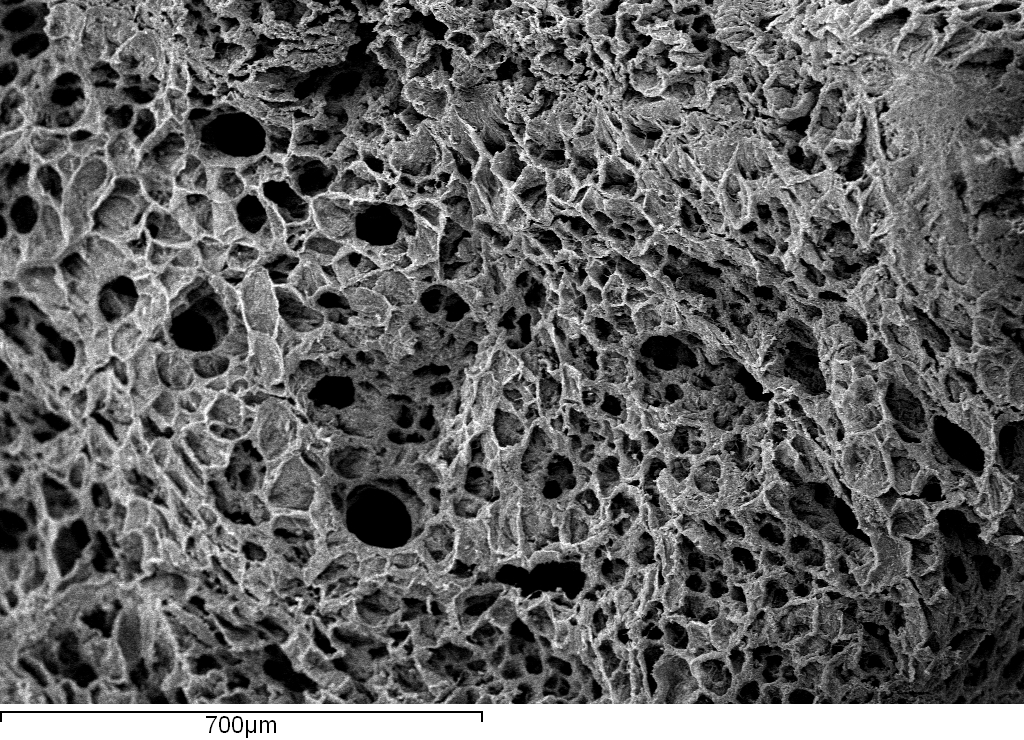
\includegraphics{figures/ratLung100X.jpg}} 
        \resizebox*{0.45\textwidth}{0.25\textheight}
        {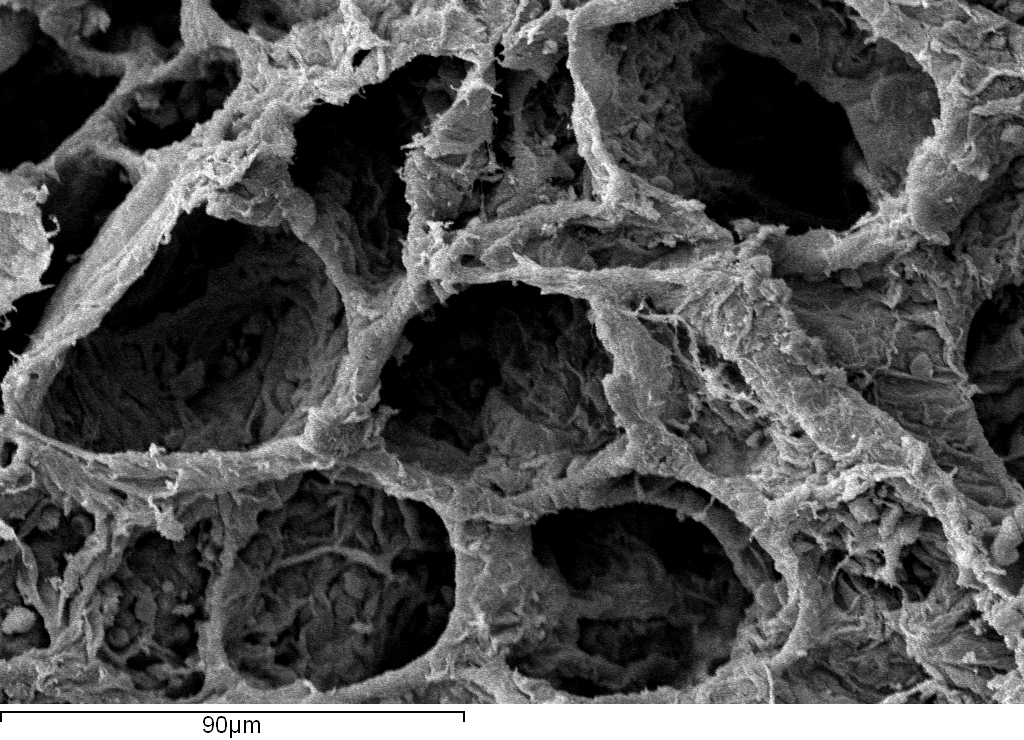
\includegraphics{figures/ratLung750X.jpg}}
        \par}
    \caption{SEM photographs from a sectioned rat lung.  Left image is at a magnification of 100X.  Right image is at a magnification of 750X. They are Figs.~5 \& 7 in Freed \textit{et~al}.\ \cite{Freedetal12}. The alveolar diameter in rat lung is about one quarter the alveolar diameter in human lung.}
    \label{figRatLung}
\end{figure}

The alveolous is modeled here using the geometry of a dodecahedron, a soccer-ball like structure comprised of twelve pentagonal facets bordered by thirty septal cords that are connected at twenty vertices, each vertex linking three neighboring cords of the alveolus with a fourth chord that extends out to neighboring alveoli.  BABT occurs, largely, through the tearing of septal cords, which affects the mechanics of breathing, and through the rupturing of capillaries traversing the alveolar facets, causing hemorrhaging thereby leading to lung contusion.  A dodecahedral model of alveoli is capable of capturing these trauma events.

\conjecture\label{conjecture}
\textit{A micro\-scopic strain field, measured at the scale of alveoli, is the same as its macro\-scopic strain field, measured at the scale of parenchyma.  Deformation is affine.}  

\medskip
This hypothesis was tested and confirmed in an experimental study done by Butler \textit{et~al}.\ \cite{Butleretal96} where they used light scattering to study changes in geometry of the septal planes in alveoli from which they concluded: ``the micro\-scopic strain field does not differ significantly from the macro\-scopic field.''  We employ this hypothesis by taking the deformation gradient from, say, a Gauss point in a finite element model of lung, and imposing it as a far-field deformation onto our dodecahedral model of an alveolus.  From this kinematic input we determine a macro\-scopic stress response homogenized from the micro\-scopic forces created within this structural model for alveoli.

The authors of a review article on alveolar strain finished by writing:
\begin{quotation}
    \noindent\small ``In general, computational mechanics approaches to determine function in a healthy or diseased lung have proven to be useful in explaining or measuring observations that are not captured by imaging modalities. However, for these models to fully explain complex physiological mechanical events, appropriate mechanical properties, boundary conditions, and mechanical loads must be identified. Moreover, validation of such computational models, which is an essential component of any computational mechanics approach, remains to be a challenge in the analysis of soft tissue mechanics.''
    
    \nopagebreak
    \mbox{} \hfill Roan \& Waters \cite[pg.~L633]{RoanWaters11} \normalsize
\end{quotation}
In this research we set out to develop a constitutive framework for alveolar mechanics, fully cognizant of the aforementioned challenges.  Our objectives are different from those of prior studies in alveolar mechanics in that we seek to describe the response\slash injury of a human lung that has been subjected to a stress wave propagating across the thorax region caused by an impact from either a blunt object or a blast wave.  Consequently, some important aspects in the modeling of a breathing lung are thought to be less impactful here, e.g., the effect of surfactant in keeping alveoli from collapsing at the end of expiration.

As a foundation, we adopt the guideline:
\begin{quotation}
	\noindent\small ``Constitutive equations are phenomenological. They are regarded as empirical by experimenters, and axiomatic by mathematicians.  In biomechanics, we often try to derive them on the basis of micro\-structure $\ldots$ in order to gain a better understanding, or to get some guidance to the mathematical form.''
	
	\nopagebreak
	\mbox{} \hfill Y.-C.~Fung \cite[pg.~431]{Fung90} \normalsize
\end{quotation}
The approach adopted here is to use the geometry of a dodecahedron as a \textit{micro\/}scopic mechanical model for alveoli, whose far-field response to mechanical stimuli, in accordance with Conjecture~\ref{conjecture}, will be used to inform the development of a \textit{macro\/}scopic mechanical model for parenchyma \cite{ClaytonFreed19}, the predominant tissue in lung.  This is deemed necessary because of the complex porous structure of parenchyma, as compared with the homo\-geneous structure of rubbery elastic solids whose theories have historically been employed to model parenchyma \cite{Fung75,Fungetal78,Vawteretal79,Fung88}.  The ARL-WMRD continuum (macroscopic) model for parenchyma \cite{ClaytonFreed19} will be implemented into finite element codes with an end application being improved and more effective designs for protective body armor. 

\section{Organization}

This document is organized in the following manner.  Part~\ref{partDodecahedron} introduces the dodecahedron as a model for alveoli.  Its geometric properties are derived in detail with regards to its three geometric features: 1D septal chords, 2D septal membranes, and 3D volume.  Part~\ref{partKinematics} develops the kinematics required for us to model a deforming dodecahedron, again focusing on the 1D~chords, 2D~membranes, and the 3D~volume within.  Part~\ref{partConstitutive} derives constitutive models suitable for describing the thermo-mechanical response for the structural constituents of an alveolus: its septal chords, its permeable membranes, and its volume.  Part~\ref{partNumericalMethods} presents numerical methods used for solving first-order parabolic and second-order hyperbolic, ordinary, differential equations (ODEs), and for solving spatial integrations along a bar, across a pentagon, and throughout a tetrahedron using Gaussian quadrature schemes designed for each geometry.  Part~\ref{partVariational} describes a variational formulation used to create our structural model of an alveolus, which consists of three models: one comprised of septal chords, another comprised of septal membranes, and the third comprised of alveolar volume.  All interpolate their stresses to the vertices where the forces from each are summed and homogenized for return to the macroscopic solver.  The first appendix provides an overview of implicit constitutive equations used in our alveolar model.  The remaining appendices provide a reference manual for the software developed to accomplish this project's objective, which was written in Python vs.~3.7.
